\section{実験結果と考察}
\label{sec:results}

\subsection{ラベル追従性}

各モデルについて，ラベルと実際のプレース変位の相関を図\,\ref{fig:label_scatter} および表\,\ref{tab:monotone} に示す．

\begin{table*}[t]
  \centering
  \caption{ラベル追従性（決定係数 $R^2$ および Spearman 相関 $\rho$）}
  \label{tab:monotone}
  \small
  \begin{tabular}{lcccc}
    \hline
    Model & $R^2$（$c_x$） & $R^2$（$c_y$） & $\rho$（$c_x$） & $\rho$（$c_y$） \\
    \hline
    \texttt{Direct w/ image}    & 0.56 & 0.50 & 0.66 & 0.76 \\
    \texttt{Residual w/ image}  & \textbf{0.94} & \textbf{0.78} & \textbf{0.97} & \textbf{0.85} \\
    \texttt{Residual w/o image} & 0.72 & 0.38 & 0.84 & 0.72 \\
    \hline
  \end{tabular}
\end{table*}

\begin{figure*}[t]
  \centering
  \begin{subfigure}[b]{0.48\linewidth}
    \centering
    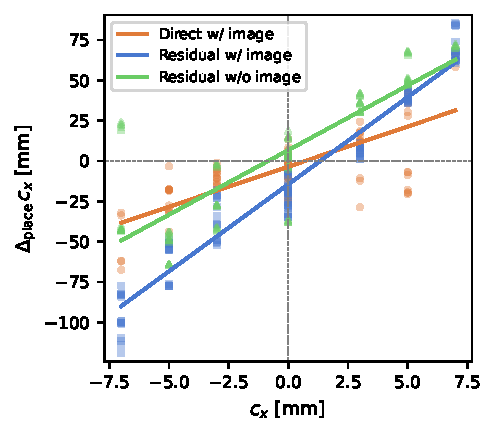
\includegraphics[width=\linewidth]{figures/fig_label_scatter_cx.pdf}
    \caption{$c_x$ 方向}
    \label{fig:label_scatter_cx}
  \end{subfigure}
  \hfill
  \begin{subfigure}[b]{0.48\linewidth}
    \centering
    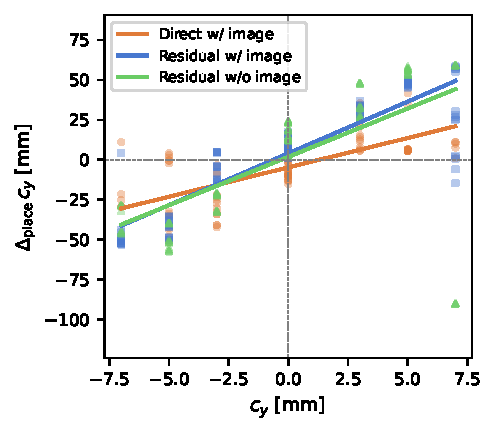
\includegraphics[width=\linewidth]{figures/fig_label_scatter_cy.pdf}
    \caption{$c_y$ 方向}
    \label{fig:label_scatter_cy}
  \end{subfigure}
  \caption{ラベルとプレース変位の関係（各モデルの散布図と回帰直線）}
  \label{fig:label_scatter}
\end{figure*}

図\,\ref{fig:label_scatter} および表\,\ref{tab:monotone} に示すように，
\texttt{Residual w/ image} は $c_x$ 方向に $\rho = 0.97$，$R^2 = 0.94$ と高い単調追従性を示した．
これは\ref{sec:method}節の仮説 --- 残差予測によって単調増加性が強まる --- を実験的に支持する結果である．
\texttt{Residual w/o image} も  $c_x$ 方向に $\rho = 0.84$，$R^2 = 0.72$ と中程度の追従性を示し，
画像なしの構成でも有効であることが確認された．
一方，\texttt{Direct w/ image} では $R^2 = 0.56$ にとどまり，
フルシーケンス予測では単調性の実現が難しいことが示された．
また $c_y$ 方向は全モデルで相関がやや低く，$c_y$ 方向の制御精度の向上が今後の課題である．

\subsection{ラベル $\bm{c} = [0,0]$ 時の系統バイアス}

ラベル $\bm{c} = [0,0]$ を与えた際の各モデルのプレース位置分布を図\,\ref{fig:bias_scatter} に示す．
モーションコピーの平均プレース位置を基準点とし，
各モデルの平均位置とのオフセットを表\,\ref{tab:bias} に示す．

\begin{figure}[t]
  \centering
  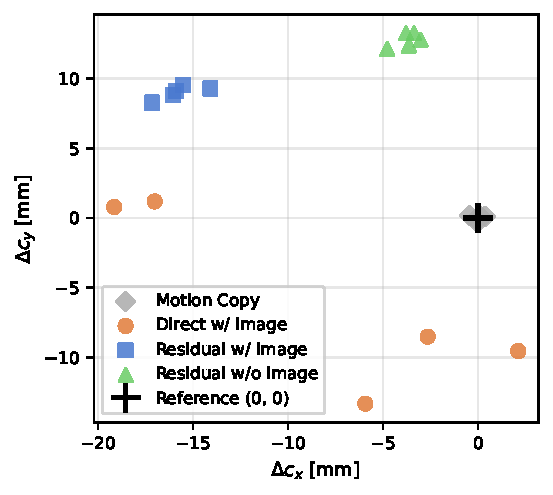
\includegraphics[width=0.92\linewidth]{figures/fig_bias_scatter.pdf}
  \caption{$\bm{c}=[0,0]$ 時のプレース位置分布．$+$ はモーションコピーの平均位置（基準点 $(0,0)$）を示す．}
  \label{fig:bias_scatter}
\end{figure}

\begin{table}[t]
  \centering
  \caption{$\bm{c}=[0,0]$ 時のプレース位置オフセットの平均値と試行間標準偏差}
  \label{tab:bias}
  \small
  \begin{tabular}{lccc}
    \hline
    Model & $n$ & offset [mm] & $\sigma_{c_x} / \sigma_{c_y}$ [mm] \\
    \hline
    \texttt{Motion Copy}        & 5 & $\approx 0$   & 0.27 / 0.19 \\
    \texttt{Direct w/ image}    & 5 & 10.3          & 8.24 / 5.83 \\
    \texttt{Residual w/ image}  & 5 & 18.1          & 0.99 / 0.43 \\
    \texttt{Residual w/o image} & 5 & 13.3          & 0.59 / 0.45 \\
    \hline
  \end{tabular}
\end{table}

\texttt{Residual w/ image} および \texttt{Residual w/o image} はそれぞれ 18.1\,mm，13.3\,mm の
系統的なオフセットが生じており，ラベル $[0,0]$ に対して残差ゼロを正確に学習できていないことを示す．
このバイアスは \texttt{Direct w/ image} の 10.3\,mm より大きく，
残差モデルの構造的な弱点といえる．
一方，試行間ばらつき（$\sigma_{c_x} / \sigma_{c_y}$）は残差モデルで $0.99 / 0.43$\,mm および $0.59 / 0.45$\,mm と
非常に小さく，\texttt{Direct w/ image} の $8.24 / 5.83$\,mm に対して高い再現性を示している．
このバイアスは，ILC ループによる反復修正で吸収できる可能性があり，今後の検証課題である．

\subsection{試行間再現性（同一ラベル内標準偏差）}

各モデルの同一ラベル内標準偏差 $\sigma_{\Delta c_x}$，$\sigma_{\Delta c_y}$ の全ラベル平均を
図\,\ref{fig:variance_bar} に示す．

\begin{figure*}[t]
  \centering
  \begin{subfigure}[b]{0.48\linewidth}
    \centering
    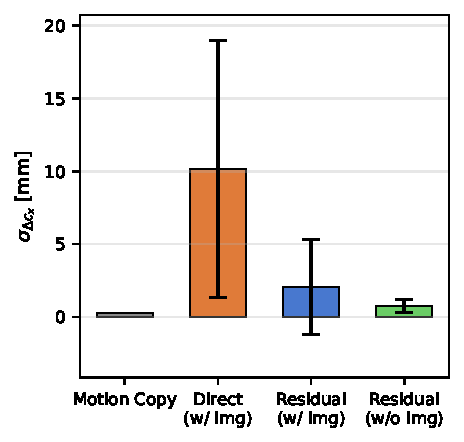
\includegraphics[width=\linewidth]{figures/fig_variance_bar_cx.pdf}
    \caption{$c_x$ 方向}
    \label{fig:variance_bar_cx}
  \end{subfigure}
  \hfill
  \begin{subfigure}[b]{0.48\linewidth}
    \centering
    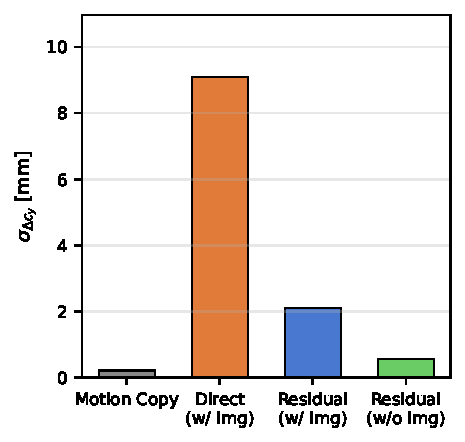
\includegraphics[width=\linewidth]{figures/fig_variance_bar_cy.pdf}
    \caption{$c_y$ 方向}
    \label{fig:variance_bar_cy}
  \end{subfigure}
  \caption{同一ラベル内プレース変位標準偏差の比較（全ラベル平均）}
  \label{fig:variance_bar}
\end{figure*}

\texttt{Motion Copy}（全ラベル平均：$\sigma_{c_x} \approx 0.30$\,mm, $\sigma_{c_y} \approx 0.21$\,mm）はハードウェア再現精度の上限を示す．なお表\,\ref{tab:bias} に示す $\sigma$ は $\bm{c}=[0,0]$ 時の 5 試行のみを対象とした値であり，測定対象が異なるため数値が若干異なる．
\texttt{Direct w/ image} はこれより 1 桁以上大きい $\sigma_{c_x} \approx 10.2$\,mm, $\sigma_{c_y} \approx 9.1$\,mm を示し，
フルシーケンス予測では推論ノイズが支配的であることが確認された．
\texttt{Residual w/ image} は $\sigma_{c_x} \approx 2.1$\,mm, $\sigma_{c_y} \approx 2.1$\,mm と \texttt{Direct w/ image} より大幅に改善されているが，
\texttt{Residual w/o image}（$\sigma_{c_x} \approx 0.75$\,mm, $\sigma_{c_y} \approx 0.57$\,mm）はさらに小さく，
モーションコピー基準に近い再現性を示した．
画像ありモデルでのばらつき増大は，照明・視点の微小変動によって画像特徴量が変動し，
推論ノイズが増大したためと考えられる．

\subsection{ピック時の手先位置偏差}

ロボットはラベル $\bm{c}$ によってプレース位置のみを変えることが意図されており，
ピック動作は全ラベルで同一であるべきである．
しかし，図\,\ref{fig:pick_pos} に示すように，すべての学習モデルでラベル値に依存したピック位置のずれが観測された．

\begin{figure*}[t]
  \centering
  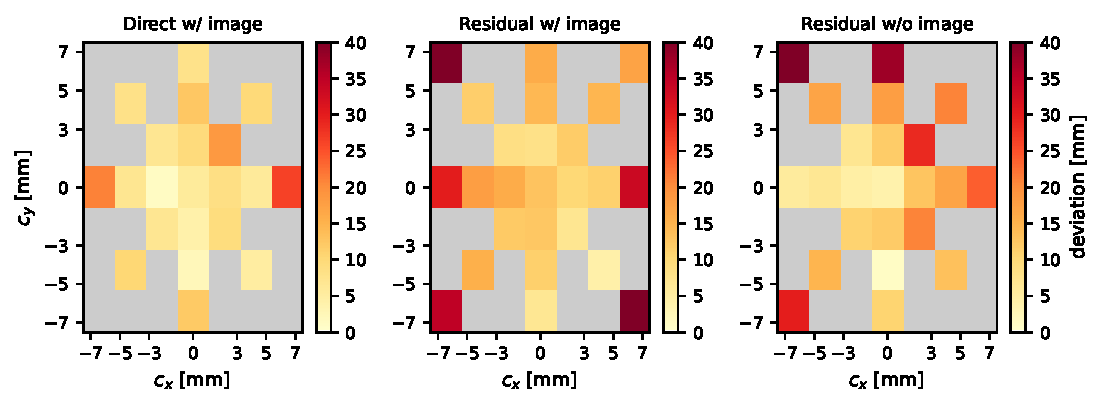
\includegraphics[width=0.92\linewidth]{figures/fig_pick_pos.pdf}
  \caption{モーションコピー平均ピック位置からのピック位置偏差ヒートマップ．灰色セルは未試行ラベルを示す．}
  \label{fig:pick_pos}
\end{figure*}

表\,\ref{tab:pick_dev} に全モデルで共通して試行した 21 ラベルにおけるピック位置偏差を示す．

\begin{table}[t]
  \centering
  \caption{ピック位置偏差（モーションコピー基準からのユークリッド距離の平均，全モデル共通の 21 ラベルで集計）}
  \label{tab:pick_dev}
  \small
  \begin{tabular}{lr}
    \hline
    Model & deviation [mm] \\
    \hline
    \texttt{Direct w/ image}    & 9.4  \\
    \texttt{Residual w/ image}  & 13.4 \\
    \texttt{Residual w/o image} & 14.1 \\
    \hline
  \end{tabular}
\end{table}

残差モデルでは \texttt{Direct w/ image} より大きいピック位置ずれが生じており，
学習した残差 $\Delta\hat{\bm{\xi}}$ がピック段階の動作にも影響を及ぼしていることが確認された．
なお，今回の共通ラベルに含まれない $\pm 7$ 対角ラベルでは，一部モデルでピック動作自体が成立しないほどの偏差が生じており，ラベル値が大きい領域でのピック干渉は特に深刻である．
理想的には残差はプレース前の特定区間にのみ作用すべきだが，
現状では動作全体に残差が加算されているため，ピック動作も変位してしまっている．
プレース区間限定の残差加算，もしくはピック・プレース動作の明示的な分離モデリングといった，ピック段階への残差干渉を抑制するためのアーキテクチャ改良が今後の課題として挙げられる．
